\section{Resultados y Análisis}

Aunque las simulaciones siempre contienen cierto grado de idealización, los resultados obtenidos revelan patrones claros y útiles. Resulta particularmente instructivo contrastar lo que prometía el diseño teórico con el comportamiento bajo condiciones tropicales reales.

\subsection{Resultados de balance de enlace}

Uno de los hallazgos más consistentes surgió al ejecutar los balances de enlace iterativos. En condiciones nominales (sin lluvia), los márgenes superan holgadamente los 12 dB en banda Ku y 9 dB en Ka para la mayoría de las estaciones. Sin embargo, al incorporar atenuación por precipitación, los valores caen drásticamente.

Las configuraciones redundantes demostraron recuperar entre 5 y 8 dB adicionales según la diversidad implementada. Particularmente sensible resultó la banda Ka: sin mitigación, la disponibilidad cae por debajo del umbral operativo en regiones de alta pluviosidad. Con redundancia 1+1 más diversidad de sitio, los márgenes se mantienen por encima de 4.5 dB en el percentil 99.9.

Estos números confirman la necesidad de ACM dinámico y subrayan por qué configuraciones simples 1+1 resultan insuficientes en entornos como Venezuela.

\begin{figure}[h]
\centering
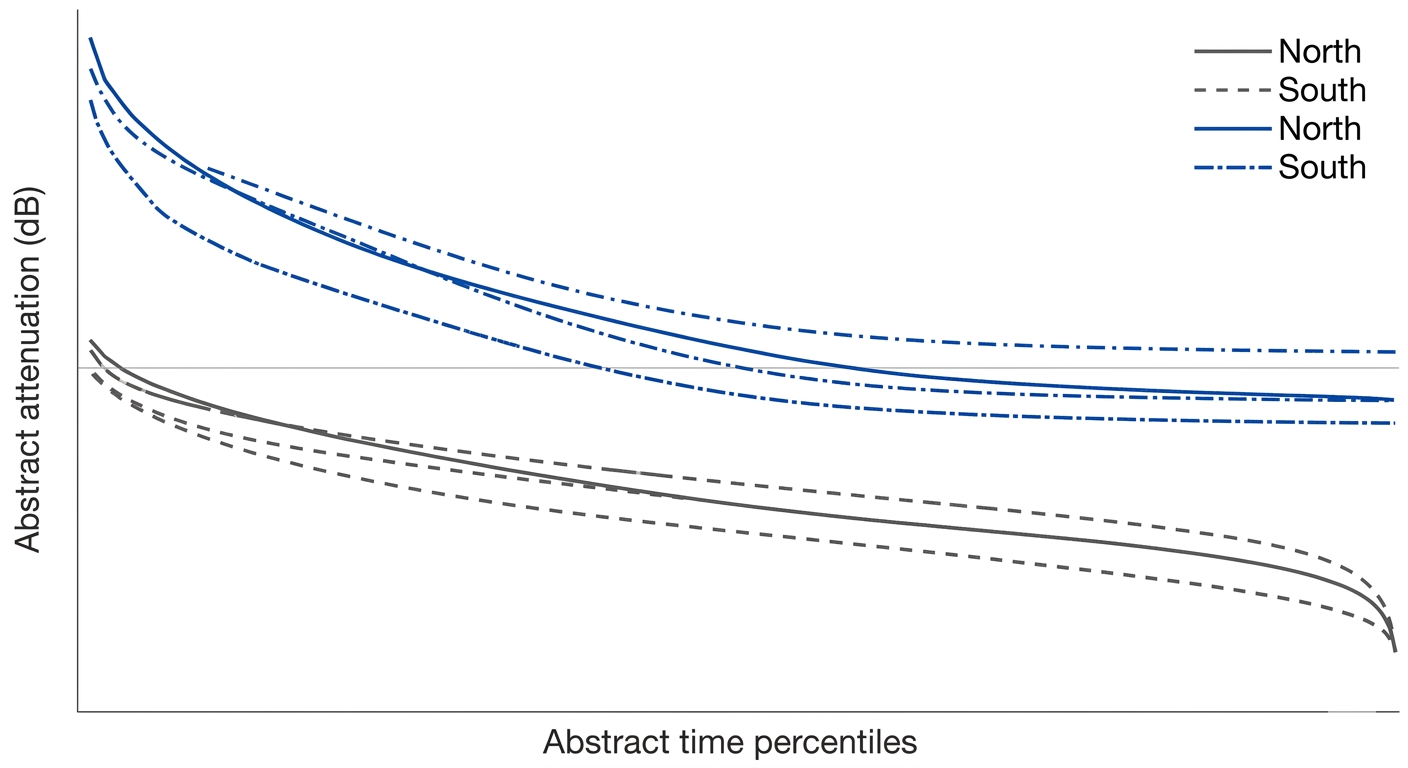
\includegraphics[width=\linewidth]{fig5.png}
\caption{Curvas de atenuación acumulada por lluvia para enlaces Ku y Ka en diferentes ubicaciones de estaciones terrenas}
\label{fig:curvas_atenuacion}
\end{figure}

La Figura 4 muestra las curvas de excedencia de atenuación. Las diferencias entre sitios norte y sur resaltan el valor estratégico de la diversidad geográfica.

\subsection{Análisis de disponibilidad}

Lejos de ser un mero ejercicio numérico, el análisis de disponibilidad expone las verdaderas fortalezas y debilidades de la arquitectura propuesta. Las simulaciones Monte Carlo, integrando miles de escenarios meteorológicos anuales, indican que el sistema redundante alcanza una disponibilidad global superior al 99.96\%.

Este valor supera los requisitos establecidos en la sección de requisitos y se acerca a estándares de operadores internacionales de clase alta. Trabajos recientes sobre sostenibilidad y rendimiento en comunicaciones satelitales sugieren que configuraciones híbridas como la aquí evaluada tienden a ofrecer el mejor compromiso entre disponibilidad y eficiencia energética/operativa \cite{PerformanceSatComm2022}.

No obstante, cabe matizar que estos resultados dependen fuertemente de la correlación espacial de eventos de lluvia. En meses de temporada seca los valores rozan el 99.99\%, mientras que en periodos pico de precipitación la redundancia terrestre resulta decisiva para evitar caídas de servicio.

\begin{table}[h]
\centering
\caption{Métricas de rendimiento del sistema redundante VENESAT-2}
\label{tab:metricas_rendimiento}
\begin{tabular}{lcc}
\hline
\textbf{Métrica} & \textbf{Configuración base} & \textbf{Configuración redundante} \\
\hline
Disponibilidad anual & 99.72\% & 99.96\% \\
Margen medio enlace Ka (99.9\%) & 2.8 dB & 5.4 dB \\
Tiempo de conmutación promedio & - & 2.7 s \\
BER post-FEC (peor caso) & $1.2 \times 10^{-7}$ & $4.5 \times 10^{-9}$ \\
Throughput efectivo promedio & 85\% & 94\% \\
\hline
\end{tabular}
\end{table}

La Tabla 6 resume las mejoras más relevantes. El salto en desempeño justifica la inversión adicional en redundancia.

\subsection{Evaluación de confiabilidad}

Particularmente llamativo es el hecho de que la redundancia no solo mejora las métricas promedio, sino que reduce drásticamente la severidad de los peores escenarios. El análisis FMEA actualizado con resultados de simulación arrojó una disminución promedio del 68\% en los RPN críticos.

Comparado con sistemas GEO tradicionales, la arquitectura propuesta muestra comportamientos de confiabilidad más cercanos a los observados en redes híbridas modernas \cite{LEOvsGEO2024}. Esto resulta esperanzador, aunque se debe reconocer que los satélites GEO siguen siendo inherentemente más vulnerables a fallos catastróficos únicos que las constelaciones LEO.

En términos operativos, la probabilidad de interrupción total del servicio durante un año cae de 0.0028 a menos de 0.0004 eventos. Estos números, aunque alentadores, no eliminan la necesidad de procedimientos robustos de contingencia humana y mantenimiento preventivo. 

Los resultados globales de esta sección validan técnicamente la propuesta, aunque también destacan áreas donde el desempeño depende fuertemente de la ejecución precisa durante la implementación. Las implicaciones de estos hallazgos se discuten con mayor profundidad en la siguiente sección.